\chapter{Time series basic metrics}
\label{sec:Chapter_metrics}
\minitoc

% \noindent Chapeau introductif
%\begin{itemize}
%	\item Rappel : notion de similaire : dans le cadre de la classification, on a un comportement « similaire » pour une même classe. La notion de « similaire » est lié à une notion de distance ou (dis)similarité. 
%	\item Donner les hypothèses de travail : 
%	\begin{itemize}
%		\item Considérons la série temporelle comme étant un objet ordonné.
%		\item les séries temporelles sont de même taille
%		\item les séries temporelles ont la même période d'échantillonnage
%		\item les séries temporelles peuvent être comparés sur l'ensemble des valeurs, sur une partie des valeurs, sur un ensemble de fenêtre (fréquences, etc.)
%	\end{itemize}
%	\item On va définir dans la suite la notion de métrique, d'alignement, de localité pour des séries temporelles.
%	\item Mettre un graphique (dit GRAPHIQUE GENERAL) qui prend 5 séries temporelles que l'on va utiliser pour la suite : proche en valeur, proche en forme, proche en fréquence, proche en valeur avec un délai, proche en forme avec un délai
%\end{itemize}

\fbox{  \parbox{0.9\textwidth}{
		In this chapter, we review different metrics for time series. In the case of classification, time series are expected to be similar if they belong to the same class. The concept of similarity among time series is directly linked to the concept of metrics. \\
		
		In the following, we consider time series as an object. We suppose that time series have the same lengths $T$ and have been sampled at the same sampling frequency $f_e$. They may be compared either on all their observations $x_{it}$, a part of them or in a window. We first recall the properties of a metric. Then, we review 3 types of metrics (amplitude-based, behavior-based, frequential-based) and kernels adapted to time series. As real time series are subjected to varying delays, we recall the concept of alignment and dynamic programming. Finally, we show how these metrics can be extended to define metrics that can capture local characteristics of time series. 
	}  }


%-----------------------------------------------------------------------------
\newpage
\section{Properties of a metric}
%\begin{itemize}
%	\item Rappeler les propriétés d'une mesure de distance (positivité, symétrique, distinguabilité, inégalité triangulaire)
%	\item Donner les différences entre métriques, distance, dissimilarités, similarités, pseudo-métrique, etc.
%	\item Dans la suite du travail, on va tout assimiler au mot métrique pour une meilleure simplicité
%\end{itemize}
A mapping $D:\mathbb{R}^T \times \mathbb{R}^T \rightarrow \mathbb{R}^+$ over a vector space $\mathbb{R}^T$ is called a metric or a distance if for all vectors $\forall \textbf{x}_i, \textbf{x}_j, \textbf{x}_l$, it satisfies the properties:
\begin{enumerate}
	\item {\makebox[6cm]{$D(\textbf{x}_i, \textbf{x}_j) \geq 0$\hfill} (positivity)}
	\item {\makebox[6cm]{$D(\textbf{x}_i, \textbf{x}_j) = D(\textbf{x}_j, \textbf{x}_i)$\hfill} (symmetry)}	
	\item {\makebox[6cm]{$D(\textbf{x}_i, \textbf{x}_j) = 0 \Leftrightarrow  \textbf{x}_i=\textbf{x}_j$\hfill} (distinguishability)}
	\item {\makebox[6cm]{$D(\textbf{x}_i, \textbf{x}_j) D(\textbf{x}_j, \textbf{x}_l) \leq D(\textbf{x}_i, \textbf{x}_l)$\hfill} (triangular inequality)}
\end{enumerate}
A mapping $D$ that satisfies properties 1, 2, 3 but not the forth one is called a dissimilarity. A mapping $D$ that satisfies properties 1, 2, 4 and not the third one is called a pseudo-metric. To simplify the discussion in the following, we refer to pseudo-metric and dissimilarity as metrics, pointing out the distinction only when necessary.

Note that for a metric, if a time series $\textbf{x}_i$ is expected to be closer to $\textbf{x}_j$ than to $\textbf{x}_l$, then $D(\textbf{x}_i,\textbf{x}_j) \leq D(\textbf{x}_i,\textbf{x}_l)$. On the contrary, when the time series $\textbf{x}_i$ is expected to be closer to $\textbf{x}_j$ than to $\textbf{x}_l$ and then $D(\textbf{x}_i,\textbf{x}_j) \geq D(\textbf{x}_i,\textbf{x}_l)$, the mapping $D$ is called a similarity.


%-----------------------------------------------------------------------------
\section{Unimodal metrics for time series}
In this section, we review 3 categories of time series metrics used in our work: amplitude-based, behavior-based and frequential-based. Let $\textbf{x}_i=(x_{i1}, x_{i2}, ..., x_{iT})$ and $\textbf{x}_j=(x_{i1}, x_{i2}, ..., x_{iT})$ be two univariate time series of length $T$. 

To illustrate the effect of different metrics, we will consider some toy examples of time series, illustrated in Fig. \ref{fig:ExampleTimeSeriesMetrics}. The objective is to determine which time series is closer to $\textbf{x}_1$. Based on the amplitude of the signals, it is straightforward that $\textbf{x}_2$ is the closest to $\textbf{x}_3$. However, if we consider the shape of the signal, $\textbf{x}_1$ is the closest to $\textbf{x}_3$. $\textbf{x}_1$ and $\textbf{x}_4$ can be considered also as the closest in value if we delete the effect of delays between the two time series. Finally, it seems that $\textbf{x}_1$ and $\textbf{x}_5$ share the same frequential components.

\begin{figure}[h!]
\centering
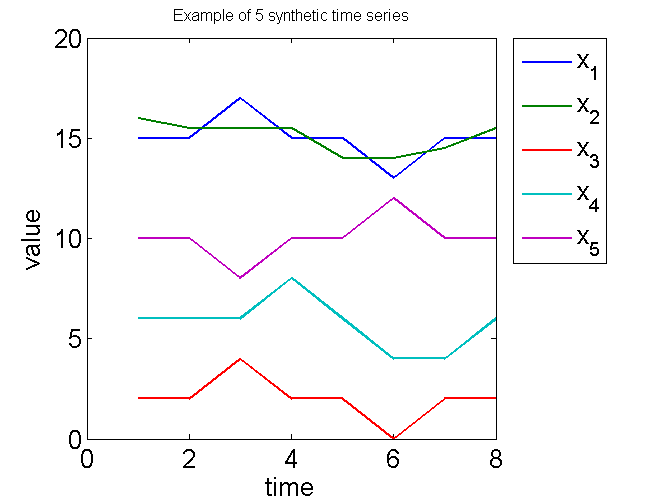
\includegraphics[width=0.6\linewidth]{images/ExampleTimeSeriesMetrics2}
\caption{An example of 4 time series that can be compared on different distinct modalities. The objective is to determine which time series is closer to $\textbf{x}_3$.}
\label{fig:ExampleTimeSeriesMetrics}
\end{figure}
\todo[  size=\tiny, color=green]{Reparler avec Michèle et Sylvain de la figure. J'aimerai pouvoir trouver 5 séries temporelles qui couvrirait ces cas.}




\subsection{Amplitude-based metrics}
\label{sec:TSmetrics}
%\begin{itemize}
%	\item Distance classiquement utilisée dans la littérature 
%	\item Distance de Minkowski (norm Lp)
%	\item Distance de Mahalanobis (norm pondéré)
%	\item $D_E$	qui est une forme particulière de Minkowski
%	\item Prendre le GRAPHIQUE GENERAL et faire le calcul des distances entre les courbes et montrer que pour 2 courbes qui ont des "amplitudes proches", on obtient une valeur de distance faible. 
%\end{itemize}

The most frequent comparison measures are amplitude-based metrics, where time series are compared in the temporal domain on their amplitudes regardless of their behaviors or frequential characteristics. Among these metrics, there are the commonly used Euclidean distance that compares elements observed at the same time \cite{Ding2008}: 
\begin{equation}	
	d_A(\textbf{x}_i,\textbf{x}_j) = \sqrt{\sum\limits_{t=1}^{T} (x_{it}-x_{jt})^2}
\label{eq:A}
\end{equation}
Note that the Euclidean distance is a particular case of the Minkowski $L_p$ norm ($p=2$). An other amplitude-based metric is the Mahalanobis distance \cite{Prekopcsak2012}:
\begin{equation}	
	d_M(\textbf{x}_i,\textbf{x}_j) = (\textbf{x}_i-\textbf{x}_j)'\textbf{M}(\textbf{x}_i-\textbf{x}_j)
	\label{eq:dM}
\end{equation}

\noindent In particular, when $\textbf{M}$ is a diagonal matrix, the previous formula becomes: 
%\textbf{M} &= 	
%\begin{pmatrix}
%	M_1 & 0 & ... & 0 \\
%	0 & M_2 & ... & 0 \\
%	... \\
%	0 & ... & & M_m 
%\end{pmatrix} \\
\begin{align}
M &= 
	\left(
	\begin{array}{ccccc}
	M_1\\
	& ... & & \text{\huge0}\\
	& & M_t & &\\
	& \text{\huge0} & & ... \\
	& & & & M_T
	\end{array}
	\right)	\\
d_M(\textbf{x}_i,\textbf{x}_j) & = \sqrt{\sum\limits_{t=1}^{T} M_t(x_{it}-x_{jt})^2}
\label{eq:dM2}
\end{align}
Intuitively, each dimension difference ($x_{it}-x_{jt}$) is weighed by a factor $M_t$. In the following of the work, we consider the standard Euclidean distance as the amplitude-based distance $d_A$.

\todo[inline]{Prendre le GRAPHIQUE GENERAL et faire le calcul des distances entre les courbes et montrer que pour 2 courbes qui ont des "amplitudes proches", on obtient une valeur de distance faible. }

\subsection{Behavior-based metrics}
%\begin{itemize}
%	\item Intuition : expliquer ce que signifie "2 séries temporelles sont proches en forme".
%	\item Dans la littérature classique, on trouve la corrélation de Pearson
%	\item Récemment, Douzal \& al. propose une généralisation: cort
%	\item Transformer la cort en mesure de dissimilarité
%	\item Prendre le GRAPHIQUE GENERAL et faire le calcul des distances entre les courbes et montrer que pour 2 courbes qui ont des "formes proches", on obtient une valeur de distance faible. 
%\end{itemize}

The second category of metrics aims to compare time series based on their shape or behavior despite the range of their amplitudes. By time series of similar behavior, it is generally intended that for all periods $[t,t']$, they increase or decrease simultaneously with the same growth rate. On the contrary, they are said of opposite behavior if for all $[t,t']$, if one time series increases, the other one decreases and (vise-versa) with the same growth rate in absolute value. Finally, time series are considered of different behaviors if they are not similar, nor opposite. Many applications refer to the Pearson correlation~\cite{Abraham2010a,Benesty2009} for behavior comparison. A generalization of the Pearson correlation is introduced in~\cite{AhlameDouzal-Chouakria2011}: 
\begin{equation}	
	cort_r(\textbf{x}_i,\textbf{x}_j) = 
	\frac{
		\sum 
		{
			(x_{it}-x_{it'})
			(x_{jt}-x_{jt'})
		}
	}
	{
		\sqrt{
			\sum 
			{(x_{it}-x_{it'})^2}
		} 
		\sqrt{
			\sum 
			{(x_{jt}-x_{jt'})^2}
		} 	 
	}
\label{eq:corTr}
\end{equation}

\noindent where $|t-t'| \leq r$, $r \in [1,..., T-1]$. \\ 

\noindent It computes the sum of growth rate between $\textbf{x}_i$ and $\textbf{x}_j$ between all pairs of values observed at $[t ,t']$ for $t' \leq t+r$ (r-order differences). The value $cort_r(\textbf{x}_i,\textbf{x}_j) = 1$ signifies that $\textbf{x}_i$ and $\textbf{x}_j$  have similar behavior. The value $cort_r(\textbf{x}_i,\textbf{x}_j) = -1$ means that $\textbf{x}_i$ and $\textbf{x}_j$ have opposite behavior. Finally, $cort_r(\textbf{x}_i,\textbf{x}_j) = 0$ expresses that their growth rates are stochastically linearly independent (different behaviors). 

When $r=1$, Eq.~\eqref{eq:corTr} leads to the temporal correlation coefficient $cort$ \cite{AhlameDouzal-Chouakria2011}. When $r=T-1$, it leads to the Pearson correlation. As $cort_r$ is a similarity measure, it can be transformed into a dissimilarity measure:
\begin{equation}
	d_B(\textbf{x}_i,\textbf{x}_j) = \frac{1 - cort_r(\textbf{x}_i,\textbf{x}_j)}{2}
	\label{eq:B}
\end{equation}

\todo[inline]{Prendre le GRAPHIQUE GENERAL et faire le calcul des distances entre les courbes et montrer que pour 2 courbes qui ont des "formes proches", on obtient une valeur de distance faible. }


\subsection{Frequential-based metrics}
%\begin{itemize}
%	\item Dans le cadre du traitement de signal, les gens utilisent des représentations fréquentielles (Fourier, etc.)
%	\item Rappeler la transformée de Fourier (TF) + spectre (module de la TF)
%	\item On peut définir une distance dans la représentation de Fourier.
%	\item Prendre le GRAPHIQUE GENERAL et faire le calcul des distances entre les courbes et montrer que pour 2 courbes qui ont des "spectres proches", on obtient une valeur de distance faible. 
%\end{itemize}
\todo[color=green]{Voir Michèle s'il faut réécrire} The third category, commonly used in signal processing, relies on comparing time series based on their frequential properties (e.g. Fourier Transform, Wavelet, Mel-Frequency Cepstral Coefficients) \cite{Sahidullah2012,Torrence1998,Brigham1967}. In our work, we limit the frequential comparison to Discrete Fourier Transform \cite{Lhermitte2011a}, but other frequential properties can be used as well. Thus, for time series comparison, first $\textbf{x}_i$ are transformed into their Fourier representation $\tilde{\textbf{x}}_i=[\tilde{x}_{i1}, ...,  \tilde{x}_{iF}]$, with $\tilde{x}_{if}$ the complex component at frequential index $f$. The Euclidean distance is then used  between their respective complex number modules $\tilde{x}_{if}$, noted $|\tilde{x}_{if}|$:
\begin{equation}
d_{F}(\textbf{x}_i,\textbf{x}_j) = \sqrt{\sum_{f=1}^{F} 
	(|\tilde{x}_{if}|-|\tilde{x}_{jf}|)^2}
\label{eq:F}
\end{equation}
\todo[inline]{Prendre le GRAPHIQUE GENERAL et faire le calcul des distances entre les courbes et montrer que pour 2 courbes qui ont des "spectres proches", on obtient une valeur de distance faible. }

\subsection{Other metrics and Kernels for time series}
\todo[inline]{A faire à la fin, pas urgent}
\begin{itemize}
	\item Il existe dans la littérature de nombreuses autres métriques pour les séries temporelles (laisser la porte ouverte).
	\item Certaines métriques sont utilisées dans le domaine temporelle
	\item D'autres métriques sont utilisés dans d'autres représentations (Wavelet, etc.)
	\item Certaines combinent la représentation temporelles et fréquentielles (Représentation spectrogramme en temps-fréquence)
	\item Se baser sur l'article "TSclust : An R Package for Time Series Clustering".
	\item Fermer le cadre : dans la suite de notre travail, on ne va pas les utiliser mais elles pourront être intégrées dans le framework qui suivra au chapitre suivant
\end{itemize}


%-----------------------------------------------------------------------------
\section{Time series alignment and dynamic programming approach}
%\begin{itemize}
%	\item Les données réelles peuvent présenter des délais, des changements de dynamique de l'échelle de temps : extension, compression (dans la limite du raisonnable).
%	\item Il existe des techniques qui permettent de ré-aligner les séries temporelles comme la DTW
%	\item Définir la notion d'alignement
%	\item Présenter la DTW (+ algorithme)
%	\item Présenter les variantes de la DTW
%	\item Dans la suite du travail, on suppose que les séries temporelles sont ré-alignées.
%	\item Prendre le GRAPHIQUE GENERAL et faire le calcul des distances entre les courbes et montrer que pour 2 courbes qui ont des "valeurs proches" mais décalés, on obtient une valeur de distance faible. (prendre DTW standard avec une fonction de coût $D_E$ par exemple)
%\end{itemize}

In some applications, time series needs to be compared at different time instants $t$ (i.e. energy data \cite{Najmeddine2012}) whereas in other applications, comparing time series on the same time instants $t$ is essential (i.e. gene expression \cite{Chouakria2007}). When time series are asynchronous (i.e. varying delays or dynamic changes), they must be aligned before any comparison or analysis process. The asynchronous effects can be of various natures: time shifting, time compression or time dilatation. For example, in the case of voice recognition (Fig. \ref{fig:Voice_Example}), it is straightforward that a same sentence said by two different speakers will produce different time series: one speaker may speak faster than the other; one speaker may take more time on some vowels, etc.

\begin{figure}[h!]
\centering
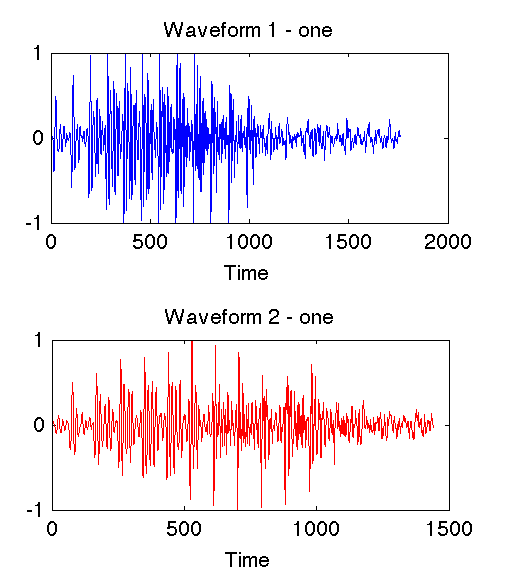
\includegraphics[width=0.4\linewidth]{images/Voice_Example}
\caption{Example of a same sentence said by two different speakers. Time series are shifted, compressed and dilatated in the time.}
\label{fig:Voice_Example}
\end{figure}
\todo[color=green]{Proposer une figure plus évidente ou plus simple?}

To cope with delays and dynamic changes, dynamic programming approach has been introduced \cite{Berndt1994a}. Let $\textbf{x}_i=(x_{i1}, ..., x_{iT})$ and $\textbf{x}_j=(x_{j1}, ..., x_{jT})$ be two time series of time length $T$. An alignment $\boldsymbol{\pi}$ of length $|\boldsymbol{\pi}|=m$ between two time series $\textbf{x}_i$ and $\textbf{x}_j$ is defined as the set of $m$ ($T \leq m \leq 2T-1$) couples of aligned elements of $\textbf{x}_i$ to $m$ elements of $\textbf{x}_j$:
\begin{equation}
\boldsymbol{\pi} = 
\left(  
(\pi_i(1),\pi_j(1)), 
(\pi_i(2),\pi_j(2)), 
\ldots,
(\pi_i(m),\pi_j(m))
\right) 
\end{equation}
\noindent where the applications $\pi_i$ and $\pi_j$ defined from $\{1, ..., m\}$ to $\{1, ..., T\}$ obey the following boundary monotonicity conditions: 
\begin{align}
& 1 = \pi_i(1) \leq \pi_i(2) \leq ... \leq \pi_i(m) = T \\
& 1 = \pi_j(1) \leq \pi_j(2) \leq ... \leq \pi_j(m) = T 
\end{align}
$\forall l \in \{1, ..., m\}$, 
\begin{align}
& \pi_i(l+1) \leq \pi_i(l)+1 \\
\text{  and  \qquad} & \pi_j(l+1) \leq \pi_j(l)+1 \\
\text{  and  \qquad} & ( \pi_i(l+1)-\pi_i(l) ) - ( \pi_j(l+1)-\pi_j(l)) \geq 1 . 
\end{align}
Intuitively, an alignment $\boldsymbol{\pi}$ defines a way to associate elements of two time series. Alignments can be described by paths in the $T \times T$ grid that crosses the elements of $\textbf{x}_i$ and $\textbf{x}_j$ (Fig. \ref{fig:DTWgrid}). We denote $\boldsymbol{\pi}$ a valid alignment and $A$, the set of all possible alignments between $\textbf{x}_i$ and $\textbf{x}_j$ ($\boldsymbol{\pi} \in A$). To find the best alignment $\boldsymbol{\pi}^*$ between two time series $\textbf{x}_i$ and $\textbf{x}_j$, the Dynamic Time Warping (\textsc{dtw}) algorithm has been proposed \cite{Keogh2004,Salvador}.

\textsc{dtw} requires to choose a cost function $\varphi$ to be optimised, such as a dissimilarity function ($d_A, d_B$, $d_F$, etc.). Classical \textsc{dtw} uses the Euclidean distance $d_E$ as the cost function~\cite{Berndt1994}. The warp path is optimize for the chosen cost function:
\begin{equation*}
\pi^* = \argmin_{\pi \in A} \frac{1}{|\boldsymbol{\pi}|}
\sum_{(t,t') \in \boldsymbol{\pi}} \varphi(x_{it}, x_{jt'})
\label{eq:DTW}
\end{equation*}

\noindent Note that when the cost function $\varphi$ is a similarity measure, the optimization involves maximization instead of minimization. The warped signal $\textbf{x}_{i,\boldsymbol{\pi}}$ and $\textbf{x}_{j,\boldsymbol{\pi}}$ are defined as:
\begin{align*}
\textbf{x}_{i,\boldsymbol{\pi}} 
&= (x_{i\pi_i(1)}, ..., 
x_{i\pi_i(m)}) 			\\	
\textbf{x}_{j,\boldsymbol{\pi}} 
&= (x_{j\pi_j(1)}, ..., 
x_{j\pi_j(m)}) 	
\end{align*}

\noindent When other constraints are applied on $\boldsymbol{\pi}$, Eq. \eqref{eq:DTW} leads to other variants of \textsc{dtw} (Sakoe-Shiba \cite{Sakoe1978a}, Itakura parallelogram \cite{Rabiner1993}).

\begin{figure}[h!]
	\centering
	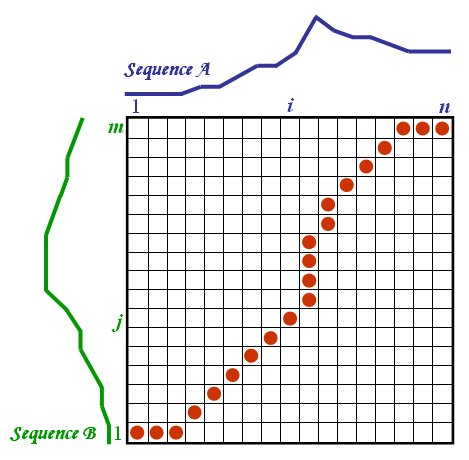
\includegraphics[width=0.4\linewidth]{images/DTWgrid}
	\caption{Example of DTW grid}
	\label{fig:DTWgrid}
\end{figure}


The previous metric (amplitude-based $d_A$, behavior-based $d_B$) can be then computed on the warped signals $\textbf{x}_{i,\boldsymbol{\pi}^*}$ and $\textbf{x}_{j,\boldsymbol{\pi}^*}$. In the following, we suppose that the best alignment $\boldsymbol{\pi}^*$ is found. For simplification purpose, we refer $\textbf{x}_{i,\boldsymbol{\pi}^*}$ and $\textbf{x}_{j,\boldsymbol{\pi}^*}$ as $\textbf{x}_{i}$ and $\textbf{x}_{j}$. 

\todo[inline]{Doit-on développer + sur la DTW comme par exemple, donner l'algorithme?}


\todo[inline]{Prendre le GRAPHIQUE GENERAL et faire le calcul des distances entre les courbes et montrer que pour 2 courbes qui ont des "valeurs proches" mais décalés, on obtient une valeur de distance faible. (prendre DTW standard avec une fonction de coût $D_E$ par exemple)}


%-----------------------------------------------------------------------------
\section{Multi-scale aspect}
%\begin{itemize}
%	\item Dans le cadre de la classification, on peut avoir des données où l'information qui permet de discriminer une classe d'une autre n'est pas globale mais est localisé sur une partie du signal
%	\item Limite des métriques basiques présentées précédemment (valeur, forme, fréquence) considère la comparaison sur l'intégralité du signal
%	\item On propose la définition de métriques locales. Pour cela, on va découper notre signal. Il existe plusieurs manières de réaliser ce découpage. On va utiliser la dichotomie proposée par Douzal \& al.
%\end{itemize}
\todo[color=green]{J'ai repris ce que ahlame avait marqué dans le papier PRL mais faudrait il réécrire?}
The systematic requisite of  the total time series elements in Eqs. \ref{eq:A}, \ref{eq:B} and \ref{eq:F},  restricts the measures potential  to capture local  temporal differences, as illustrated in Fig. \ref{fig:UMD}. This section provides a multi-scale framework for time series comparison, crucial to capture latent local, as well as global discriminative features. Many methods exist in the literature such as the dichotomy or the sliding window. We detailed here the dichotomy process used in our work.

\begin{figure}[h!]
\centering
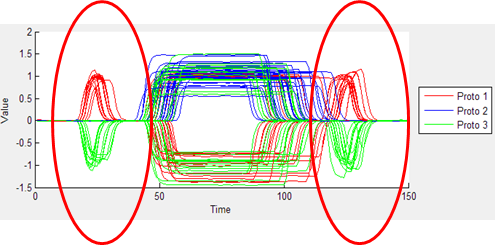
\includegraphics[width=0.7\linewidth]{images/UMD}
\caption{UMD dataset. The dataset is made of 3 classes : Up, Middle and Down. The 'Up' class has a characteristic upward bell at the beginning or at the end of the time series. The 'Down' class has a characteristic downward bell at the beginning or at the end of the time series. The 'Middle' class has no characteristic bell. Circle red show the region of interest of these bells. This region are local and standard global metric fails to show these characteristics.}
\label{fig:UMD}
\end{figure}

A multi-scale description is obtained by repeatedly segmenting a time series expressed at a given temporal scale to induce its description at a coarser level. The segmentation process refers to different approaches that mainly assume fixed either the number of the segments or their lengths. A multi-scale
comparison is then obtained by comparing time series, based on usual measures, through several segments of different temporal granularities. For a multi-scale amplitude-based comparison based on binary segmentation, Figure \ref{fig:Intervalles} shows the set of involved amplitude-based measures $d^{Is}_A$. The local behaviors- and frequential- based measures $d^{Is}_B$ and $d^{Is}_F$ are obtained similarly.

\begin{figure}[h!]
\centering
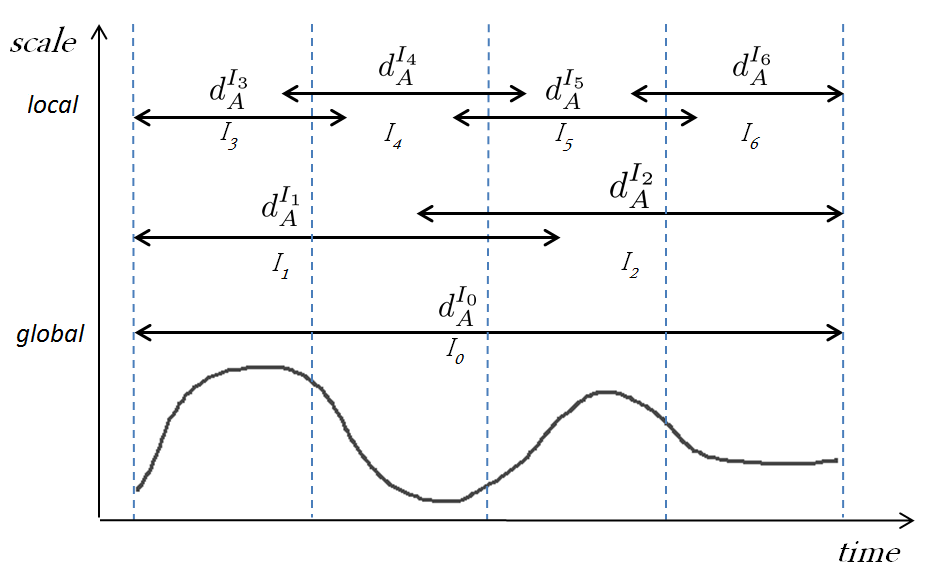
\includegraphics[width=0.7\linewidth]{images/Intervalles}
\caption{Multi-scale amplitude-based measures $d^{Is}_A$}
\label{fig:Intervalles}
\end{figure}



%-----------------------------------------------------------------------------
\newpage
\section{Conclusion of the chapter}
To cope with specificities inherent to time series, we review in this chapter several basic metrics dedicated to time series. Depending on the considered modality (amplitude, behavior, frequency), adapted metrics for time series have been proposed in the literature such as the Euclidean distance $d_A$, the Temporal correlation $d_B$ or the Fourier-based distance $d_F$.

In practice, real time series may be subjected to delays. Thus, they need to be re-aligned before any analysis task. For that, the Dynamic Time Warping (\textsc{dtw}) algorithm has been proposed. Finally, to capture local characteristics, the previous metrics $(d_A, d_B, d_F)$ can be computed on smaller intervals. Many strategies exist such as the dichotomy or the sliding window.

However, all of these metrics only include one modality and at a particular scale. Generally, several modalities may be implied. In the next chapter, we review some advanced metrics. First, we recall some combined temporal metrics that have been proposed in the literature. They mainly combine the Euclidean distance $d_A$ and the Temporal correlation $d_B$. After that, we will take an insight on Metric Learning approaches which aims to learn a metric that makes closer samples that are expected to be similar, and far away those expected to be dissimilar.


% In the next section, we present a new temporal metric learning framework for a robust nearest neighbors time series classification and give, in Section 4, a solution to learn a holistic temporal metric that combines efficiently several temporal modalities at different scales.





%%% Local Variables: 
%%% mode: latex
%%% TeX-master: "../roque-phdthesis"
%%% End: 
